In order to test Hong-Oh-Mandel interference in the lab, they added a time delay to one arm of their interferometer
\begin{figure*}[h]
	\centering
	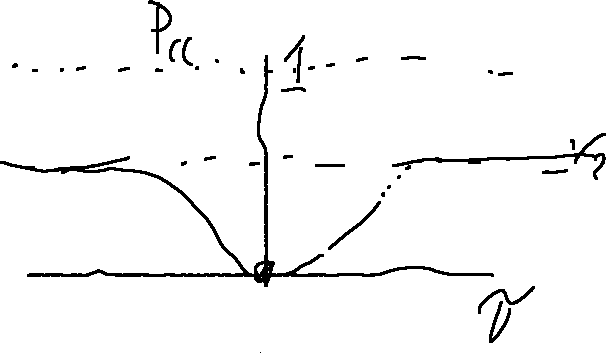
\includegraphics[width=6cm]{2-17-1.png}
	\caption*{Hong "dip"}
\end{figure*}
It can quickly be shown that the coincidence amplitude with our delay is:
\begin{align*}
	\ket{cc} &= \frac{1}{2}(\hat{a}_{4\psi}^\dagger\hat{a}_{3\phi}^\dagger -\hat{a}_{3\psi}^\dagger\hat{a}_{4\phi}^\dagger)\vac \\
	P_{cc} &= \frac{1}{4} \bra{\text{vac}}(\hat{a}_{3\phi}\hat{a}_{4\psi} -\hat{a}_{4\phi}\hat{a}_{3\psi})(\hat{a}_{4\psi}^\dagger\hat{a}_{3\phi}^\dagger -\hat{a}_{3\psi}^\dagger\hat{a}_{4\phi}^\dagger)\vac \\
	P_{cc} &= \frac{1}{4} (2 - \bra{\text{vac}}(\hat{a}_{3\phi}\hat{a}_{4\psi}\hat{a}_{3\psi}^\dagger\hat{a}_{4\phi}^\dagger - \hat{a}_{3\psi}\hat{a}_{3\phi}^\dagger\hat{a}_{4\phi}\hat{a}_{4\psi}^\dagger)\vac)
\end{align*}
We know $[\hat{a}_\psi,\hat{a}_\phi^\dagger] = (\psi|\phi) = \int \frac{d\omega}{2\pi} \tilde{\psi}^*(\omega)\tilde{\phi}(\omega)$, Therefore ($\hat{a}_{3\phi}\hat{a}_{3\psi}^\dagger = \hat{a}_{3\psi}^\dagger\hat{a}_{3\phi} + (\psi|\phi)$:
\begin{align*}
	P_{cc} &= \frac{1}{4} (2 - 2\Re{\bra{\text{vac}} [\hat{a}_{3\psi}^\dagger\hat{a}_{3\phi} + (\psi|\phi)][\hat{a}_{4\phi}^\dagger\hat{a}_{4\psi} + (\phi|\psi)]}) \\
	P_{cc} &= \frac{1}{4} (2 - 2|(\phi|\psi)|^2)
\end{align*}
If we assume we have a gaussian temporal mode, then we expect this term to go as $e^{-\frac{\tau^2}{T^2}}$, which is exactly what was observed in Hong Oh and Mandel's experiment. Clearly we would expect our two photon rates to be the compliment of the 1 photon rates.

We now turn our attention to visibility in interference effects. We define the visibility of an interferometer as $\frac{I_\text{max} - I_\text{min}}{I_\text{max} + I_\text{min}}$.
For a classical Michaelson interferometer, we predict a unit visibility, but many practical effects limit this, such as mismatched losses in the arms. This gives us a visibility of $\frac{2\tau}{1+\tau^2}$.
In the quantum sense this can be though of as introducing distinguishability between the two paths. This can additionally be introduced by changing the mode of light as it passes through one of the paths.
In our Hong mandel interference we can talk about our visibility as $\frac{P_{cc}(\infty) - P_{cc}(0)}{P_{cc}(\infty)}$. For Hong-Oh-Mandel this is $|(\phi|\psi)|^2$.

We can talk about single photons in terms of single photon density operators:
\begin{align*}
	\hat{\rho} &= \sum_m \ket{1}_{\psi m}\bra{1}_{\psi m} p_m
\end{align*}
Which when this is the input to both sides of the interferometer will give us a visibility of $1-\Tr{\hat{\rho}^2}$.
Post selection using measurement on only one port gives us a non-linear interaction. This is the basis of linear-optics quantum computing.

\subsection{Two mode squeezed vacuum}
We introduce our new squeezing operator:
\begin{align*}
	\hat{S}_{12}(\xi) &= e^{\xi^* \hat{a}_1\hat{a}_2 - \xi\hat{a}_1^\dagger\hat{a}_2^\dagger}
\end{align*}
Where these two modes are fully orthogonal. Our two mode squeezed vaccuum state is:
\begin{align*}
	\ket{\text{TMSV}_\xi}_{12} &= \hat{S}_{12} (\xi)\vac
\end{align*}
We now look at this state in term of different representations of it. Clearly we know that our two modes must always have the same number of photons.

We first look at our quadratures:
\begin{align*}
	\hat{q}_\pm &= \frac{\hat{q}_1 \pm \hat{q}_2}{2} \\
	\hat{p}_\pm &= \frac{\hat{p}_1 \pm \hat{p}_2}{2}
\end{align*}
And we can see that our commutators are simply:
\begin{align*}
	[\hat{q}_+,\hat{p}_+] &= \frac{i}{2} \\
	[\hat{q}_-,\hat{p}_-] &= \frac{i}{2} \\
	[\hat{q}_+,\hat{p}_-] &= 0 \\
	[\hat{q}_-,\hat{p}_+] &= 0
\end{align*}
We say:
\begin{align*}
	\hat{S}_{12}^\dagger(\xi)\hat{a}_1\hat{S}_{12}(\xi) &= \hat{a}_1\cosh r - e^{i\theta} \hat{a}_2^\dagger\sinh r \\
	\hat{S}_{12}^\dagger(\xi)\hat{a}_2\hat{S}_{12}(\xi) &= \hat{a}_2\cosh r - e^{i\theta}\hat{a}_1^\dagger \sinh r
\end{align*}
So:
\begin{align*}
	\expval{\hat{q}_+} &= \bra{\text{vac}}\hat{S}_{12}^\dagger(\xi)\hat{q}_+\hat{S}_{12}(\xi)\vac \\
	\expval{\hat{q}_+} &= 0
\end{align*}
But:
\begin{align*}
	\expval{\hat{q}_+^2} &= \bra{\text{vac}}\hat{S}_{12}^\dagger(\xi)\hat{q}_+\hat{S}_{12}(\xi)\hat{S}^\dagger_{12}(\xi)\hat{q}_+\hat{S}_{12}(\xi)\vac
\end{align*}
Where we can show (for a certain choice of $\theta$):
\begin{align*}
	\hat{S}^\dagger\hat{q}_+\hat{S} &= q_1\cosh r - q_2\sinh r
\end{align*}
So then:
\begin{align*}
	\expval{\hat{q}_+^2} &= \frac{1}{4} e^{-2r} \\
	\expval{\hat{p}_+^2} &= \frac{1}{4} e^{2r}
\end{align*}
We can now look at these operators in order to find our number representation, which is:
\begin{align*}
	\ket{\xi}_{12} &= \frac{1}{\cosh r} \sum_n (-1)^n e^{in\theta}(\tanh r)^n \ket{n}_1\ket{n}_2
\end{align*}
This can be thought of the result of a two mode spontaneous parametric down conversion (SPDC).

Clearly:
\begin{align*}
	\expval{\hat{n}_1 - \hat{n}_2} &= 0 \\
	\expval{\hat{n}_1} &= \sinh^2 r
\end{align*}
We can also see:
\begin{align*}
	\hat{\rho}_1 &=\Tr_2\{\ket{\xi}_{12}\bra{\xi}_{12}\} \\
	\hat{\rho}_1 &=\sum_m |\lambda|^{2n}\ket{m}_1\bra{m}_1
\end{align*}
Which has thermal statistics!
